\documentclass[12pt]{article}                         
\pagestyle{plain}

\usepackage{amsmath}     % Enhanced math environments (e.g., align).
\usepackage{amsfonts}    % Math fonts (e.g., \mathfrak{}).
\usepackage{amstext}     % Text inside math mode (e.g., \text{where}).
\usepackage{amssymb}     % Extra math symbols (e.g., \mathbb{R}).
\usepackage{array}       % Advanced table/array column definitions.
\usepackage{circledtext} % Puts text inside a circle (e.g., \circledtext{A}).
\usepackage{comment}     % Include/exclude blocks of text.
\usepackage{enumerate}   % Customize itemized/numbered lists.
\usepackage{graphicx}    % Include images/graphics (\includegraphics).
\usepackage{latexsym}    % Access to basic LaTeX symbols.
\usepackage{multicol}    % Allows text columns on a page.
\usepackage{pgfplots}    % Create scientific plots from data (based on TikZ).
\usepackage{tabularx}    % Tables that stretch to page width.
\usepackage{tasks}       % Create multi-column lists.
\usepackage{textcomp}    % Provides many text symbols (e.g., \textcelsius).
\usepackage{tikz}        % Create vector graphics and diagrams.
\usepackage{xcolor}      % Define and use colors.
\usepackage{fancyhdr}
\usepackage{tcolorbox}
\usepackage{enumitem}

\usepackage[
  letterpaper,
  left=0.8in,
  right=0.8in,
  textheight=9.5in,
  bmargin=0.5in  % Adjust this value to push the footer down
]{geometry}
\pagestyle{fancy}
\fancyhf{} % Clear all header and footer fields
\fancyhead[L]{Your Name:} % Left header with name
\fancyhead[R]{November 13th 2025} % Right header with date
\renewcommand{\headrulewidth}{0.4pt} % Horizontal line below the header

\begin{document}

% Main title
\begin{center}
    \Large \textbf{Math 115E Activity 18} \\
    \vspace{0.2cm}
    \normalsize Chapter 6 \\
    \normalsize Transformations
\end{center}
\vspace{-0.5cm}
\noindent
\section*{Transformation Rules}
\begin{table}[h!]
\centering
\begin{tabular}{|c|c|c|c|}
\hline
\textbf{Function} & \textbf{Vertical Translation} & \textbf{Result} & \textbf{Point} \\
\hline
$y = x^2$ & \textbf{Upward} by $k$ units & $y = x^2 + k$ & $(x, y + k)$ \\
\hline
$y = x^2$ & \textbf{Downward} by $k$ units & $y = x^2 - k$ & $(x, y - k)$ \\
\hline
$y = x^2$ & \textbf{Right} by $h$ units & $y = (x - h)^2$ & $(x - h, y)$ \\
\hline
$y = x^2$ & \textbf{Left} by $h$ units & $y = (x + h)^2$ & $(x + h, y)$ \\
\hline
$y = x^2$ & \textbf{Stretch} for $|c|\geq 1$ & $y = 2f(x)$ & $(x, 2y)$ \\
\hline
$y = x^2$ & \textbf{Shrink} for $0<|c|<1$ & $y = \frac{1}{2}f(x)$ & $(x, \frac{1}{2}y)$ \\
\hline
$y = x^2$ & \textbf{Reflection} over the $x-axis$ & $y = -x^2$ & $(x, -y)$ \\
\hline
$y = x^2$ & \textbf{Reflection} over the $y-axis$ & $y = (-x)^2$ & $(-x, y)$ \\
\hline
\end{tabular}
\end{table}


\section*{Quadratic Function Transformations}

% The tabular environment uses fixed-width columns (p{}) to ensure text wrapping.
% The vertical height is enforced using \rule{0pt}{5cm} inside the second data row.
Convert each of the following Transformations from function notation into descriptive words \\\\
\begin{tabular}{|>{\centering\arraybackslash}p{4cm}|>{\centering\arraybackslash}p{4cm}|>{\centering\arraybackslash}p{4cm}|>{\centering\arraybackslash}p{4cm}|}
\hline
$y = \displaystyle\frac{1}{2}f(x-1)+2$ & $y=5f(x)+3$ & $y=-2f(x+1)-2$ & $y=f(x-3)+4$ \\
% This row contains the large vertical gap, enforced by \rule{0pt}{5cm}
& \rule{0pt}{8cm}& &  \\
\hline
\end{tabular}

%% ADD REFLECTIONS TO THE TABLE
\noindent
\section*{Transformations From Graph}
\begin{minipage}[c]{0.40\textwidth} % Minipage for all graphs
    \centering

    % === GRAPH 1 ===
    Adjust $y=f(x)$ below with transformation $y=2f(x)$
    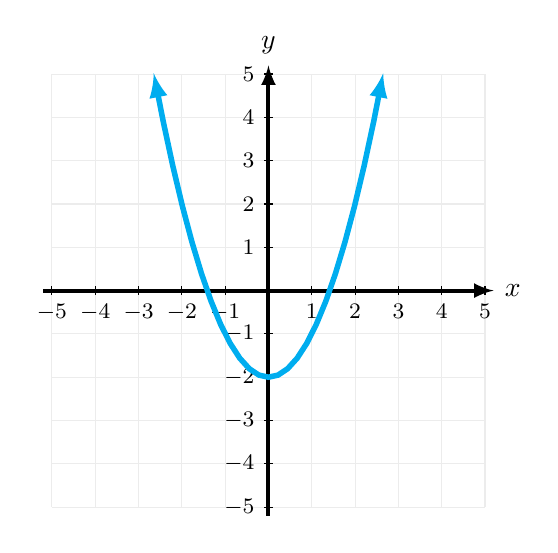
\begin{tikzpicture}
	[
		scale=0.55,
		vector style/.style={->, very thick}
	]
    \draw[gray!15,step=1cm] (-5,-5) grid (5,5);
        \draw[line width=0.5mm, -latex] (-5.2,0) -- (5.2,0) node[right] {$x$};
        \foreach \x in {-5,-4,-3,-2,-1,1,2,3,4,5} \draw (\x,.1)--(\x,-.1) node[below] {\footnotesize $\x$};
        \draw[line width=0.5mm,  -latex] (0,-5.2) -- (0,5.2) node[above] {$y$};
        \foreach \y in {-5,-4,-3,-2,-1,1,2,3,4,5} \draw (.1,\y)--(-.1,\y) node[left] {\footnotesize $\y$};
        \draw[cyan,line width=2pt,latex-latex] plot[domain= -2.65:2.65] (\x,{\x*\x-2});
    \end{tikzpicture}

    \vspace{0.5cm} % Add some space between graphs

    % === GRAPH 2 ===
    Adjust $y=h(x)$ below with transformation $y=h(x-3)$
    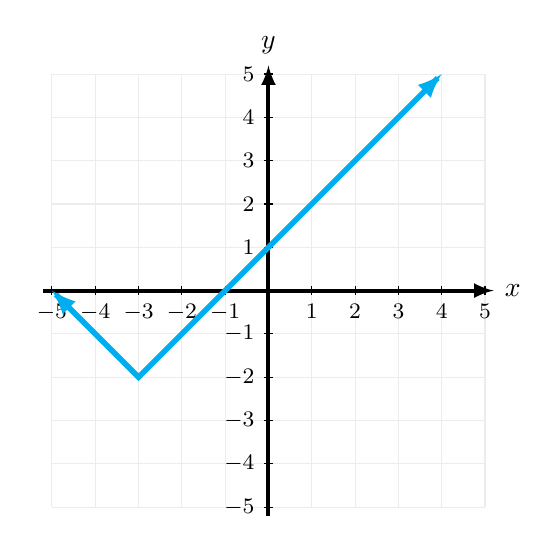
\begin{tikzpicture}
	[
		scale=0.55,
		vector style/.style={->, very thick}
	]
    \draw[gray!15,step=1cm] (-5,-5) grid (5,5);
        \draw[line width=0.5mm, -latex] (-5.2,0) -- (5.2,0) node[right] {$x$};
        \foreach \x in {-5,-4,-3,-2,-1,1,2,3,4,5} \draw (\x,.1)--(\x,-.1) node[below] {\footnotesize $\x$};
        \draw[line width=0.5mm,  -latex] (0,-5.2) -- (0,5.2) node[above] {$y$};
        \foreach \y in {-5,-4,-3,-2,-1,1,2,3,4,5} \draw (.1,\y)--(-.1,\y) node[left] {\footnotesize $\y$};
        \draw[cyan,line width=2pt,latex-latex] plot[domain= -5:4, samples=100] (\x,{abs(\x + 3) - 2});
    \end{tikzpicture}

    \vspace{0.5cm} % Add some space between graphs

    % === GRAPH 2 ===
    Adjust $y=h(x)$ below with transformation $y=h(x-3)$
    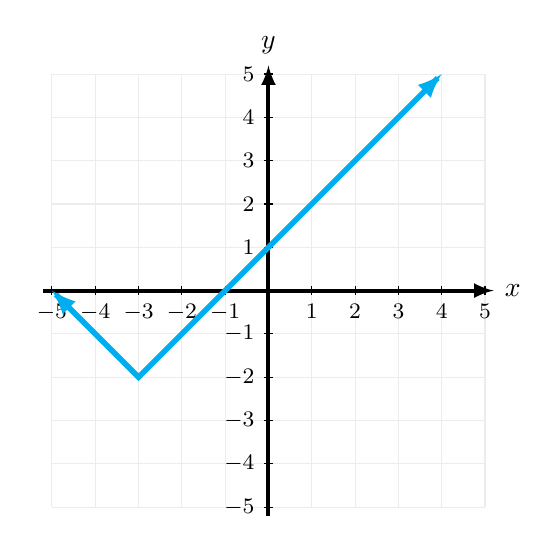
\begin{tikzpicture}
	[
		scale=0.55,
		vector style/.style={->, very thick}
	]
    \draw[gray!15,step=1cm] (-5,-5) grid (5,5);
        \draw[line width=0.5mm, -latex] (-5.2,0) -- (5.2,0) node[right] {$x$};
        \foreach \x in {-5,-4,-3,-2,-1,1,2,3,4,5} \draw (\x,.1)--(\x,-.1) node[below] {\footnotesize $\x$};
        \draw[line width=0.5mm,  -latex] (0,-5.2) -- (0,5.2) node[above] {$y$};
        \foreach \y in {-5,-4,-3,-2,-1,1,2,3,4,5} \draw (.1,\y)--(-.1,\y) node[left] {\footnotesize $\y$};
        \draw[cyan,line width=2pt,latex-latex] plot[domain= -5:4, samples=100] (\x,{abs(\x + 3) - 2});
    \end{tikzpicture}

\end{minipage}
\hfill
\begin{minipage}[c]{0.40\textwidth} % Minipage for all graphs
    \centering

    % === GRAPH 4 ===
    Adjust $y=g(x)$ below with transformation $y=-g(x)$
    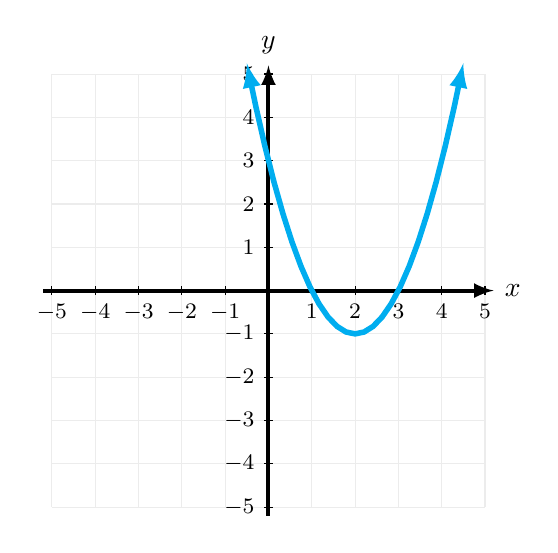
\begin{tikzpicture}
	[
		scale=0.55,
		vector style/.style={->, very thick}
	]
    \draw[gray!15,step=1cm] (-5,-5) grid (5,5);
        \draw[line width=0.5mm, -latex] (-5.2,0) -- (5.2,0) node[right] {$x$};
        \foreach \x in {-5,-4,-3,-2,-1,1,2,3,4,5} \draw (\x,.1)--(\x,-.1) node[below] {\footnotesize $\x$};
        \draw[line width=0.5mm,  -latex] (0,-5.2) -- (0,5.2) node[above] {$y$};
        \foreach \y in {-5,-4,-3,-2,-1,1,2,3,4,5} \draw (.1,\y)--(-.1,\y) node[left] {\footnotesize $\y$};
        \draw[cyan,line width=2pt,latex-latex] plot[domain= -0.5:4.5] (\x,{((\x-2)^2) - 1});
    \end{tikzpicture}

    \vspace{0.5cm} 

    % === GRAPH 5 ===
    Adjust $y=k(x)$ below with transformation $y=-k(x)-3$
    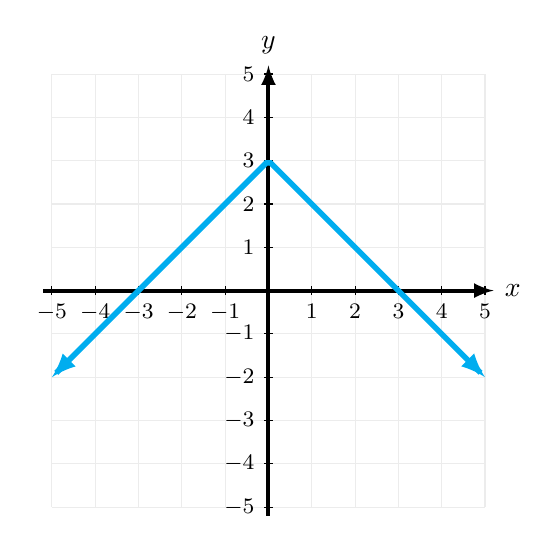
\begin{tikzpicture}
	[
		scale=0.55,
		vector style/.style={->, very thick}
	]
    \draw[gray!15,step=1cm] (-5,-5) grid (5,5);
        \draw[line width=0.5mm, -latex] (-5.2,0) -- (5.2,0) node[right] {$x$};
        \foreach \x in {-5,-4,-3,-2,-1,1,2,3,4,5} \draw (\x,.1)--(\x,-.1) node[below] {\footnotesize $\x$};
        \draw[line width=0.5mm,  -latex] (0,-5.2) -- (0,5.2) node[above] {$y$};
        \foreach \y in {-5,-4,-3,-2,-1,1,2,3,4,5} \draw (.1,\y)--(-.1,\y) node[left] {\footnotesize $\y$};
        \draw[cyan,line width=2pt,latex-latex] plot[domain= -5:5, samples=100] (\x,{-1*abs(\x) + 3});
    \end{tikzpicture}

    \vspace{0.5cm} 

    % === GRAPH 6 ===
    Adjust $y=k(x)$ below with transformation $y=-k(x)-3$
    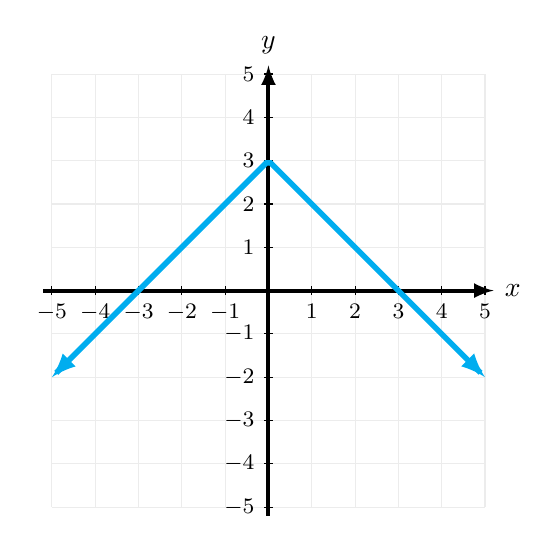
\begin{tikzpicture}
	[
		scale=0.55,
		vector style/.style={->, very thick}
	]
    \draw[gray!15,step=1cm] (-5,-5) grid (5,5);
        \draw[line width=0.5mm, -latex] (-5.2,0) -- (5.2,0) node[right] {$x$};
        \foreach \x in {-5,-4,-3,-2,-1,1,2,3,4,5} \draw (\x,.1)--(\x,-.1) node[below] {\footnotesize $\x$};
        \draw[line width=0.5mm,  -latex] (0,-5.2) -- (0,5.2) node[above] {$y$};
        \foreach \y in {-5,-4,-3,-2,-1,1,2,3,4,5} \draw (.1,\y)--(-.1,\y) node[left] {\footnotesize $\y$};
        \draw[cyan,line width=2pt,latex-latex] plot[domain= -5:5, samples=100] (\x,{-1*abs(\x) + 3});
    \end{tikzpicture}

    

\end{minipage}
\end{document}